\documentclass{standalone}
\usepackage[utf8]{inputenc}
\usepackage{amsmath}
\usepackage{amsfonts}
\usepackage{amssymb}
\usepackage{tikz}
\usetikzlibrary{calc}

% GanttHeader setups some parameters for the rest of the diagram
% #1 Width of the diagram
% #2 Width of the space reserved for task numbers
% #3 Width of the space reserved for task names
% #4 Number of months in the diagram
% In addition to these parameters, the layout of the diagram is influenced
% by keys defined below, such as y, which changes the vertical scale
\def\GanttHeader#1#2#3#4{%
 \pgfmathparse{(#1-#2-#3)/(#4)}
 \tikzset{y=7mm, task number/.style={left, font=\bfseries},
     task description/.style={text width=#3,  right, draw=none,
           font=\sffamily, xshift=#2,
           minimum height=2em},
     gantt bar/.style={draw=black, fill=blue!30},
     help lines/.style={draw=black!30, dashed},
     x=\pgfmathresult pt
     }
  \def\totalmonths{#4}
  \node (Header) [task description] at (0,0) {\textbf{\large }};
  \begin{scope}[shift=($(Header.south east)$)]
    \foreach \x in {1,...,#4}
      \node[above,rotate=90] at (\x,1) {\tiny\x};
 \end{scope}
}

% This macro adds a task to the diagram
% #1 Number of the task
% #2 Task's name
% #3 Starting date of the task (month's number, can be non-integer)
% #4 Task's duration in months (can be non-integer)
\def\Task#1#2#3#4{%
%\node[task number] at ($(Header.west) + (0, -#1)$) {#1};
\node[task description] at (0,-#1) {#2};
\begin{scope}[shift=($(Header.south east)$)]
  \draw (0,-#1) rectangle +(\totalmonths, 1);
  \foreach \x in {1,...,\totalmonths}
    \draw[help lines] (\x,-#1) -- +(0,1);
  \filldraw[gantt bar] ($(#3, -#1+0.2)$) rectangle +(#4,0.6);
\end{scope}
}

\begin{document}

\begin{tabular}{lr}
Scheduler: & RR-3 scheduler
\\
Input: & input/testdata3.txt
\\
Total Process Count: & 17
\\
Total Waiting Time: & 2055
\\
Average Waiting Time: & 120.882355
\\
Total Turnaround Time: & 2259
\\
Average Turnaround Time: & 132.88235
\\
Total Context Switch Count: & 73
\\
\end{tabular}
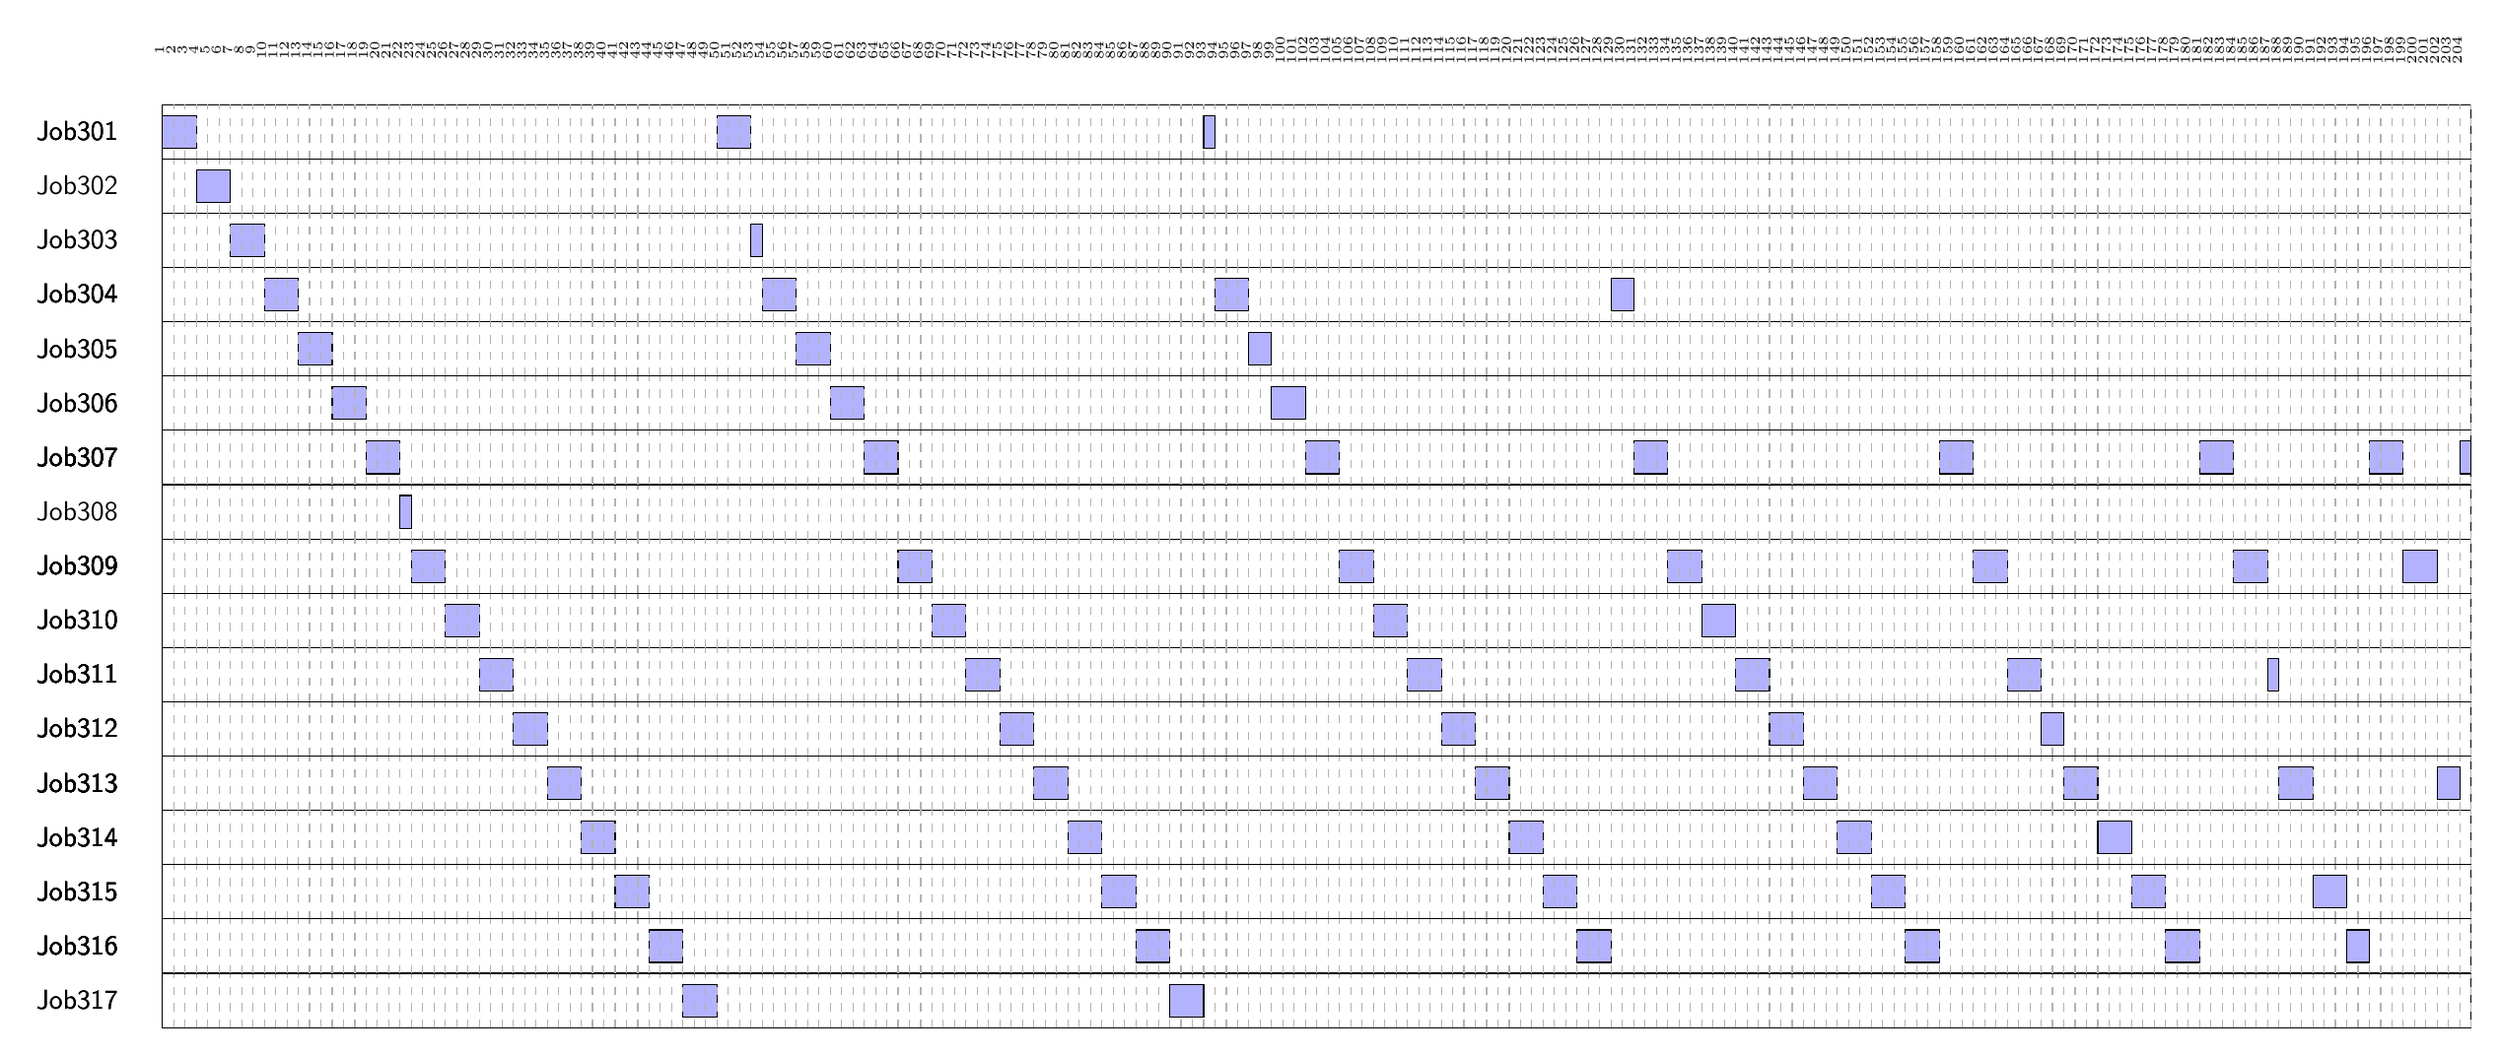
\begin{tikzpicture}
\GanttHeader{32cm}{5ex}{1.5cm}{204}
\Task{1}{Job301}{0}{3}
\Task{2}{Job302}{3}{3}
\Task{3}{Job303}{6}{3}
\Task{4}{Job304}{9}{3}
\Task{5}{Job305}{12}{3}
\Task{6}{Job306}{15}{3}
\Task{7}{Job307}{18}{3}
\Task{8}{Job308}{21}{1}
\Task{9}{Job309}{22}{3}
\Task{10}{Job310}{25}{3}
\Task{11}{Job311}{28}{3}
\Task{12}{Job312}{31}{3}
\Task{13}{Job313}{34}{3}
\Task{14}{Job314}{37}{3}
\Task{15}{Job315}{40}{3}
\Task{16}{Job316}{43}{3}
\Task{17}{Job317}{46}{3}
\Task{1}{Job301}{49}{3}
\Task{3}{Job303}{52}{1}
\Task{4}{Job304}{53}{3}
\Task{5}{Job305}{56}{3}
\Task{6}{Job306}{59}{3}
\Task{7}{Job307}{62}{3}
\Task{9}{Job309}{65}{3}
\Task{10}{Job310}{68}{3}
\Task{11}{Job311}{71}{3}
\Task{12}{Job312}{74}{3}
\Task{13}{Job313}{77}{3}
\Task{14}{Job314}{80}{3}
\Task{15}{Job315}{83}{3}
\Task{16}{Job316}{86}{3}
\Task{17}{Job317}{89}{3}
\Task{1}{Job301}{92}{1}
\Task{4}{Job304}{93}{3}
\Task{5}{Job305}{96}{2}
\Task{6}{Job306}{98}{3}
\Task{7}{Job307}{101}{3}
\Task{9}{Job309}{104}{3}
\Task{10}{Job310}{107}{3}
\Task{11}{Job311}{110}{3}
\Task{12}{Job312}{113}{3}
\Task{13}{Job313}{116}{3}
\Task{14}{Job314}{119}{3}
\Task{15}{Job315}{122}{3}
\Task{16}{Job316}{125}{3}
\Task{4}{Job304}{128}{2}
\Task{7}{Job307}{130}{3}
\Task{9}{Job309}{133}{3}
\Task{10}{Job310}{136}{3}
\Task{11}{Job311}{139}{3}
\Task{12}{Job312}{142}{3}
\Task{13}{Job313}{145}{3}
\Task{14}{Job314}{148}{3}
\Task{15}{Job315}{151}{3}
\Task{16}{Job316}{154}{3}
\Task{7}{Job307}{157}{3}
\Task{9}{Job309}{160}{3}
\Task{11}{Job311}{163}{3}
\Task{12}{Job312}{166}{2}
\Task{13}{Job313}{168}{3}
\Task{14}{Job314}{171}{3}
\Task{15}{Job315}{174}{3}
\Task{16}{Job316}{177}{3}
\Task{7}{Job307}{180}{3}
\Task{9}{Job309}{183}{3}
\Task{11}{Job311}{186}{1}
\Task{13}{Job313}{187}{3}
\Task{15}{Job315}{190}{3}
\Task{16}{Job316}{193}{2}
\Task{7}{Job307}{195}{3}
\Task{9}{Job309}{198}{3}
\Task{13}{Job313}{201}{2}
\Task{7}{Job307}{203}{1}
\end{tikzpicture}
\end{document}
